\documentclass[11pt]{article}
%\usepackage{html}
\usepackage{graphicx}
\newcommand{\comments}[1]{}

\begin{document}
\begin{center}
{\Large \bf  E84 Midterm Exam 1 --- Fall 2015}
\end{center}

{\bf Instructions}
\begin{itemize}
\item Write your name on top of each page. Indicate the total number of 
  pages submitted.
\item When solving a problem, list the main steps. In each step describe 
  very concisely what you are doing, then show the calculation and the 
  result of the step. A final answer, even if correct, without evidence 
  of the steps leading to the answer will receive no credit. 
\item Put all answers in the spaces provided, show your steps and 
  calculation on separate sheets.
\end{itemize}

\newpage

{\bf The Problems}
\begin{enumerate}

\item {\bf Problem 2. (60 points)} 
  In the figure below, $V_1=20V$, $V_2=10V$, $I=2A$, $R_1=R_2=10\Omega$, 
  $R_3=6\Omega$, $R_5=R_6=2.5\Omega$, $R_4=1.5\Omega$.
  \begin{itemize}
    \item {\bf (20 pts)} 
      Voltage $V_{ab}$ (+ on left, - on right):

      $V_{ab}=$\underline{\hspace{2cm}V}

  \end{itemize}
    
  \begin{itemize}
  \item {\bf (20 pts)} 
    Currents $I_1$, $I_2$, $I_3$, $I_4$, $I_5$, and $I_6$ (all assumed
    to flow down or rightward) through $R_1$, $R_2$, $R_3$, $R_4$, $R_5$, 
    and $R_6$, respectively:    

    $I_1=$\underline{\hspace{2cm}A },$\;\;\;\;\;\;$
    $I_2=$\underline{\hspace{2cm}A },$\;\;\;\;\;\;$
    $I_3=$\underline{\hspace{2cm}A },$\;\;\;\;\;\;$
    $I_4=$\underline{\hspace{2cm}A },$\;\;\;\;\;\;$
    $I_5=$\underline{\hspace{2cm}A },$\;\;\;\;\;\;$
    $I_6=$\underline{\hspace{2cm}A }

  \item {\bf (20 pts)}
    Find a new value of $R_2$ for current through it to be $I_2=1$ A:

    $R_2=$\underline{\hspace{2cm}$\Omega$}
  \end{itemize}

\begin{figure}[h!]
\centering
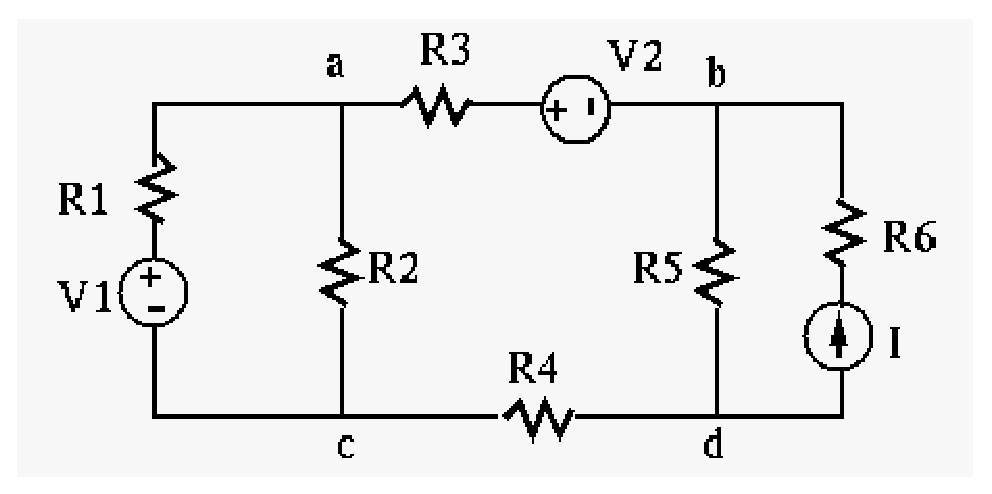
\includegraphics[scale=0.5]{midterm12015f.eps}
%\caption{The SOM network}
%\label{Fig1}
\end{figure}

\comments{
{\bf Solution:} Use Thevenin's theorem. 
\begin{itemize}
\item Remove $R_3$ and $V_3$ as the load
\item Convert $I$ and $R_5$ to a voltage source $V_3=5V$ with $R_5=2.5$.
\item Find open-circuit voltage $V_T$:
  \[
  V_{ab}=V_a-V_b=V_1\frac{R_5}{R_1+R_5}-V_3=20 \frac{10}{10+10}-5=5 
  \]
\item Find $R_T$:
  \[
  R_T=R_1//R_2+R_4+R_5=5+1.5+2.5=9
  \]
\item Connect load of $V_3$ and $R_3$, find current $I_3$:
  \[
  I_3=\frac{V_T-V_3}{R_T+R_3}=\frac{5-10}{9+6}=-\frac{1}{3} 
  \]
\item Find $V_{ab}$ 
  \[
  V_{ab}=-\frac{1}{3}\times 6 +10=8V
  \]
\item $I_4=-I_3=1/3$, $I_5=2-1/3=5/6$.
\item $V_{dc}=I_4R_4=1.5/3=-0.5V$, $V_{bd}=R_5I_5=2.5\,(5/6)=25/6$,
  $V_{ac}=V_{ab}+V_{bd}+V_{dc}=8+25/6-0.5=35/3$, $I_2=V_{ac}/R_2=7/6$
\item Treat $R_2$ as load, find Thevenin's model for the two parallel
  branches: $V_1=20$ in series with $R_1=10$, and $V_2+V_3=10+5=15$ in
  series with $R_3+R_4+R_5=1.5+2.5+6=10$. Convert them into two current
  sources with $I_a=V_1/R_1=2A$ and $I_b=15/10=1.5A$. Combine these 
  parallel branches: $I_a+I_b=3.5A$, $R_1//(R_3+R_4+R_5)=10//10=5$.
  Convert this current source to a voltage source of $V_T=17.5$ and
  $R_T=3.5$. $I_2=V_T/(R_T+R_2)=17.5/15=7/6$ (same as before).
\item For the current $I_2=V_T/(R_T+R_2)=17.5/(5+R_2)=1$ to be 1, 
  $R_2=12.5$.
\end{itemize}

}

\newpage

\item {\bf Problem 2. (40 points)} 
In the circuit below, $I_0=6A$, $V_0=5V$, $R_1=2\Omega$, $R_2=R_4=4\Omega$, 
$R_3=8\Omega$. Find the current $I_5$ through $R_5=6\Omega$:

$I_5=$\underline{\hspace{2cm}A }

\begin{figure}[h!]
\centering
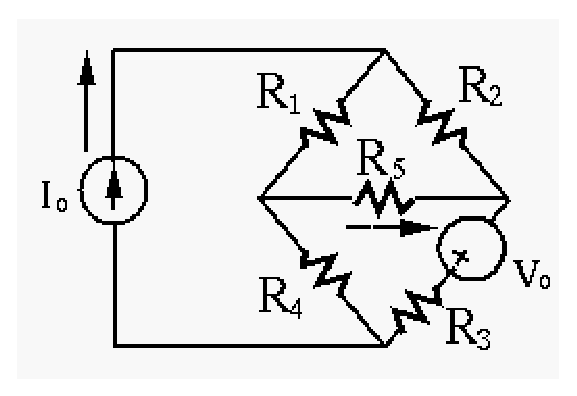
\includegraphics[scale=0.6]{midterm1f.eps}
%\caption{The SOM network}
%\label{Fig2}
\end{figure}

\comments{
{\bf Solution:} Use superposition. First consider the current source $I_0$ 
only with $V_0=0$ (short-circuit). Convert the delta composed of the top three 
resistors ($R_1$, $R_2$ and $R_5$) to Y:
\[
R_a=\frac{2\times 4}{2+6+4}=\frac{2}{3},\;\;\;\;
R_b=\frac{2\times 6}{2+6+4}=1,\;\;\;\;R_c=\frac{4\times 6}{2+6+4}=2 
\]
where $R_a$ is in series with $I_0$, and $R_b$ and $R_c$ are in series with 
$R_4$ and $R_3$, respectively. Treating the two branches as two voltage dividers,
we find the voltage across $R_5$ is zero and therefore $I'=0$,

Next consider the voltage source $V_0$ only, with $I_0=0$ (open-circuit).
The total resistance of the loop is 
\[
R_3+R_4+R_5//(R1+R_2)=8+4+6//(2+4)=15\Omega
\]
and the total current is 
\[
I_{total}=\frac{5V}{15\Omega}=\frac{1}{3}\;A
\]
and the current through $R_5$ can be found by current divider to be 
\[
I''=I_{total}=\frac{1}{3}\frac{R_1+R_2}{R_5+R_1+R_2}=\frac{1}{6}\;A
\]
The current due to both $I_0$ and $V_0$ is therefore $I=I'+I''=1/6\;A$.

Alternatively, we use Thevenin's model:
\begin{itemize}
\item Find $R_T$
  \[
  R_T=(R_1+R_2)//(R_3+R_4)=6//12=72/18=4
  \]
\item Find $V_T$ (+ on right) by superposition:
  $V'_T$ due to $V_0$ alone:
  \[
  V'_T=V_0\frac{R_1+R_2}{R_1+R_2+R_3+R_4}=5\frac{6}{18}=\frac{5}{3}
  \]
  $V''_T=0$ due to $I_0$ alone, because $R1/R_4=R_2/R_3$
\item 
  \[
  I=\frac{V_T}{R_T+R_5}=\frac{5}{3}\frac{1}{4+6}=\frac{1}{6}
  \]
\end{itemize}
}

\end{enumerate}

\end{document}

